\section{Deskriptivní statistická analýza. Popis, agregace a komparace ekonomických dat}

\subsection*{Smysl deskriptivní statistické analýzy}
\term{Deskriptivní statistická analýza} popisuje data tak, aby bylo zřejmé, co se v nich stalo,
v jaké velikosti, struktuře, čase a mezi jakými skupinami. Nejde o dokazování kauzality ani o predikci
budoucnosti. Cílem je shrnout realitu zachycenou v datech a připravit podklad pro interpretaci,
reporting, další modelování nebo rozhodnutí.

Typické otázky:
\begin{itemize}
  \item kolik jednotek, zákazníků, transakcí nebo událostí data obsahují;
  \item jaká je typická hodnota ukazatele;
  \item jak moc jsou hodnoty rozptýlené;
  \item zda je rozdělení symetrické, šikmé, vícemodální nebo zatížené odlehlými hodnotami;
  \item jak se ukazatel liší podle regionu, času, produktu, kanálu nebo segmentu;
  \item jak se změnil proti plánu, minulému období nebo benchmarku.
\end{itemize}

Deskriptivní analýza je základní vrstva business intelligence i exploratorní analýzy. V BI poskytuje
metriky a KPI pro reporty a dashboardy. V exploratorní analýze pomáhá odhalit strukturu dat, chyby,
extrémy a proměnné vhodné pro další zpracování.

\term{Hromadný jev} je skutečnost, která se vyskytuje u mnoha jednotek nebo opakovaně v čase, takže
má smysl ji popisovat statisticky. \term{Statistický ukazatel} je číselná charakteristika takového
jevu: musí mít jasný věcný obsah, jednotku, územní a časové vymezení a výpočetní pravidlo. Například
tržby za měsíc, míra nezaměstnanosti nebo průměrná mzda nejsou jen čísla, ale ukazatele s konkrétní
definicí.

\subsection*{Typy proměnných a volba statistiky}
Volba statistiky závisí na typu proměnné. Jinak se popisuje kategorie produktu, spokojenost na škále
1--5 a peněžní hodnota objednávky.

\begin{center}
\small
\begin{tabular}{@{}>{\raggedright\arraybackslash}p{0.22\textwidth}
                >{\raggedright\arraybackslash}p{0.31\textwidth}
                >{\raggedright\arraybackslash}p{0.36\textwidth}@{}}
\hline
\term{Typ proměnné} & \term{Příklad} & \term{Vhodný popis} \\
\hline
Nominální & region, pohlaví, produktová kategorie & četnosti, relativní četnosti, modus,
kontingenční tabulka \\
Ordinální & spokojenost 1--5, rating, pořadí & četnosti, kumulativní četnosti, medián,
kvantily \\
Intervalová & teplota ve stupních Celsia, skóre & průměr, směrodatná odchylka, rozdíly,
histogram \\
Poměrová & tržby, náklady, počet kusů, čas trvání & průměr, medián, rozptyl, indexy,
tempa růstu, poměrové ukazatele \\
\hline
\end{tabular}
\end{center}

U ekonomických dat je důležité rozlišovat také jednotku měření a smysl nuly. Tržby v Kč mají
přirozenou nulu a lze počítat poměry. Teplota ve stupních Celsia přirozenou nulu nemá, a proto
věta \uv{20 stupňů je dvakrát více než 10 stupňů} nedává smysl.

Ekonomické ukazatele lze členit také podle času a konstrukce. \term{Okamžikové} ukazatele popisují
stav k určitému datu, například zásoby k poslednímu dni měsíce. \term{Intervalové} ukazatele popisují
tok za období, například měsíční tržby. \term{Primární} ukazatele jsou přímo zjištěné, zatímco
\term{sekundární} vznikají výpočtem, například podílem, rozdílem nebo indexem.

\subsection*{Četnostní analýza}
\term{Četnostní analýza} shrnuje, jak často se v datech vyskytují jednotlivé hodnoty nebo kategorie.
Používá se hlavně pro nominální a ordinální proměnné, ale také pro kvantitativní hodnoty rozdělené
do intervalů.

Základní pojmy:
\begin{itemize}
  \item \term{absolutní četnost} \(n_j\) - počet výskytů kategorie \(j\);
  \item \term{relativní četnost} \(p_j = n_j/n\) - podíl kategorie na celku;
  \item \term{kumulativní četnost} - postupný součet četností v uspořádaných kategoriích;
  \item \term{modus} - nejčastější hodnota nebo kategorie.
\end{itemize}

Příklad: u objednávek lze spočítat počet objednávek podle stavu \texttt{nova}, \texttt{zaplacena},
\texttt{stornovana}. U ratingu spokojenosti lze navíc sledovat kumulativní podíl zákazníků, kteří
hodnotili nejvýše určitou známkou.

\subsection*{Míry polohy}
\term{Míry polohy} popisují typickou nebo centrální hodnotu proměnné.

\term{Aritmetický průměr}:
\[
  \bar{x} = \frac{1}{n}\sum_{i=1}^{n}x_i.
\]
Je vhodný pro metrická data s rozumně symetrickým rozdělením a bez silných extrémů. Je citlivý na
odlehlé hodnoty: několik mimořádně velkých objednávek může zvýšit průměrnou hodnotu objednávky,
i když většina objednávek je běžná.

\term{Vážený průměr}:
\[
  \bar{x}_w = \frac{\sum_{i=1}^{n} w_i x_i}{\sum_{i=1}^{n} w_i}.
\]
Používá se, pokud pozorování nemají stejnou váhu. V ekonomických datech je typické vážit cenu
prodaným množstvím, marži tržbami nebo výběrové šetření designovými vahami. Častá chyba je počítat
průměr z průměrů bez ohledu na velikost skupin.

\term{Geometrický průměr} se hodí pro průměrování koeficientů růstu a násobných změn. Pokud hodnota
roste postupně o různé procentní změny, průměrné tempo růstu se nepočítá aritmetickým průměrem
procent, ale přes geometrický průměr růstových koeficientů.

\term{Harmonický průměr} se používá u poměrů, kde je přirozené průměrovat převrácené hodnoty, například
u rychlostí nebo jednotkových cen při pevně daném objemu. \term{Chronologický průměr} se používá pro
časové řady okamžikových stavů, například průměrný stav zásob nebo počet zaměstnanců během období.

\term{Medián} je prostřední hodnota po seřazení dat. Polovina pozorování je menší nebo rovna mediánu
a polovina větší nebo rovna. Medián je robustnější vůči extrémům než průměr, proto se často používá
u příjmů, cen nemovitostí, délek čekání nebo hodnot objednávek s dlouhým pravým ocasem.

\term{Modus} je nejčastější hodnota. U kategoriálních proměnných je často nejpřirozenější mírou
polohy. U spojitých dat se obvykle interpretuje přes histogram jako nejhustší oblast.

\term{Kvantily} dělí seřazená data podle pořadí. Medián je 50\% kvantil. Kvartily \(Q_1\), \(Q_2\)
a \(Q_3\) odpovídají přibližně 25\%, 50\% a 75\% hodnot. Decily dělí data na deset částí, percentily
na sto částí. V ekonomii se kvantily používají například pro popis příjmového rozdělení, cenových
pásem nebo zákaznických segmentů.

\begin{figure}[htbp]
  \centering
  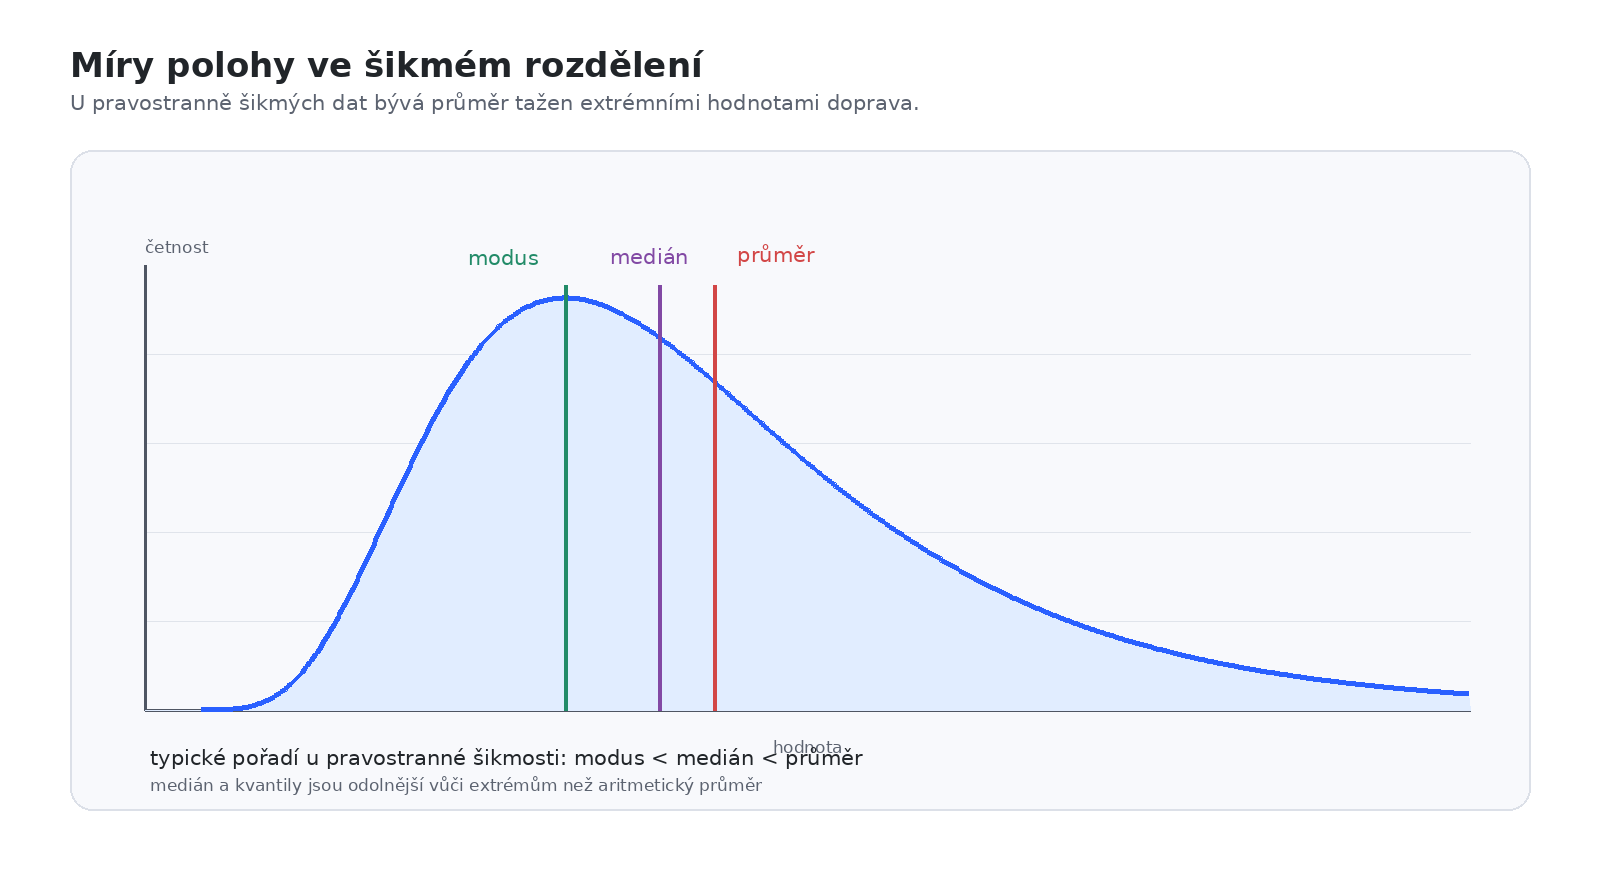
\includegraphics[width=0.95\linewidth]{assets/images/deskriptivni-statistika/mean-median-skewness.png}
  \caption[Míry polohy ve šikmém rozdělení]{Průměr, medián a modus ve šikmém rozdělení. Popis obrázku:
  pravostranně šikmá křivka ukazuje, že průměr je tažen delším pravým ocasem, zatímco medián a modus
  zůstávají blíže hlavní koncentraci hodnot. Zdroj obrázku: vlastní schéma podle obecných vlastností
  měr polohy.}
  \label{fig:mean-median-skewness}
\end{figure}

\subsection*{Míry variability}
\term{Variabilita} popisuje, jak moc se hodnoty liší. Dvě skupiny mohou mít stejný průměr, ale úplně
jinou stabilitu. Pro řízení firmy je často rozdíl mezi průměrem a variabilitou zásadní: stabilní
proces s menším rozptylem může být hodnotnější než proces se stejným průměrem, ale velkými výkyvy.

\term{Rozpětí}:
\[
  R = x_{\max} - x_{\min}.
\]
Je jednoduché, ale závisí jen na dvou extrémních hodnotách.

\term{Rozptyl} a \term{směrodatná odchylka}:
\[
  s^2 = \frac{1}{n-1}\sum_{i=1}^{n}(x_i-\bar{x})^2,
  \qquad
  s = \sqrt{s^2}.
\]
Rozptyl měří průměrnou čtvercovou odchylku od průměru. Směrodatná odchylka vrací měřítko do původních
jednotek. Obě míry jsou citlivé na extrémy, protože odchylky jsou umocněné.

\term{Interkvartilové rozpětí}:
\[
  IQR = Q_3 - Q_1.
\]
Popisuje šířku prostředních 50\% hodnot. Je robustnější vůči extrémům než rozpětí a směrodatná odchylka.

\term{Variační koeficient}:
\[
  CV = \frac{s}{\bar{x}}.
\]
Vyjadřuje relativní variabilitu vůči průměru. Hodí se pro porovnání variability ukazatelů v různých
jednotkách nebo s různou úrovní, například tržeb dvou produktů. Smysl má hlavně pro kladná poměrová
data a nenulový průměr.

\subsection*{Boxplot a odlehlé hodnoty}
\term{Boxplot} neboli krabicový graf shrnuje rozdělení pomocí mediánu, kvartilů, IQR, vousů a
potenciálních odlehlých hodnot. Je vhodný hlavně pro porovnání kvantitativní proměnné mezi skupinami,
například hodnoty objednávky podle kanálu nebo mzdy podle regionu.

Tukeyho pravidlo pro označení potenciálních odlehlých hodnot:
\[
  x < Q_1 - 1{,}5IQR
  \quad \text{nebo} \quad
  x > Q_3 + 1{,}5IQR.
\]
Přísnější hranice používá \(3IQR\). Tyto hranice neznamenají, že se má hodnota automaticky smazat.
Outlier může být chyba, ale také důležitý obchodní případ, podvod, výpadek, VIP zákazník nebo změna
procesu.

\begin{figure}[htbp]
  \centering
  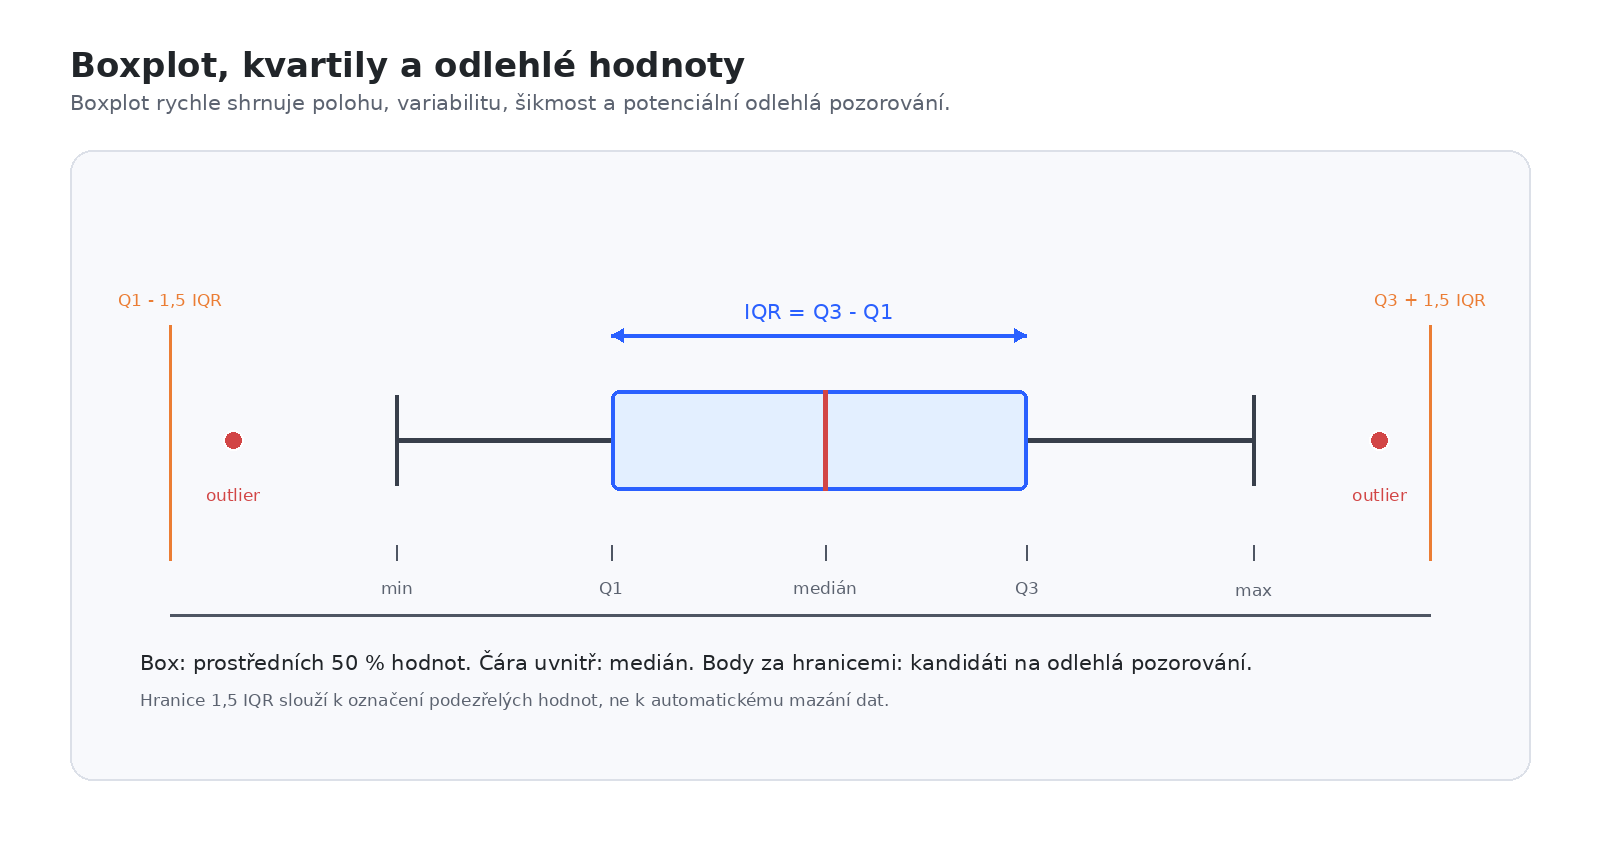
\includegraphics[width=0.95\linewidth]{assets/images/deskriptivni-statistika/boxplot-iqr-outliers.png}
  \caption[Boxplot a IQR]{Boxplot, kvartily a potenciální odlehlé hodnoty. Popis obrázku: krabice
  reprezentuje prostředních 50\% hodnot, čára uvnitř medián, vousy běžný rozsah a body za hranicemi
  1,5 IQR kandidáty na odlehlá pozorování. Zdroj obrázku: vlastní schéma podle Tukeyho boxplotu.}
  \label{fig:boxplot-iqr-outliers}
\end{figure}

\subsection*{Tvar rozdělení}
Kromě polohy a variability se sleduje \term{tvar rozdělení}. Ten je důležitý pro interpretaci statistik
i pro výběr dalších metod.

\term{Šikmost} popisuje asymetrii rozdělení. Pravostranně šikmé rozdělení má dlouhý pravý ocas,
typicky u příjmů, tržeb zákazníků nebo čekacích dob. Levostranně šikmé rozdělení má dlouhý levý ocas.
U pravostranné šikmosti často platí průměr \(>\) medián.

\term{Špičatost} nebo \term{kurtóza} popisuje těžkost ocasů vůči referenčnímu rozdělení. V praxi je
důležité hlavně vědět, zda jsou v datech těžké ocasy a extrémy. Různé softwary používají různé
konvence: někde má normální rozdělení kurtózu 3, jinde se používá nadměrná kurtóza, kde má normální
rozdělení hodnotu 0.

Graficky se tvar rozdělení kontroluje histogramem, boxplotem, hustotou, případně Q-Q grafem. Samotná
tabulka průměru a směrodatné odchylky může podstatnou strukturu skrýt.

\subsection*{Agregace dat}
\term{Agregace} je shrnutí detailních dat na vyšší úroveň. Z transakcí na úrovni položky objednávky
lze například vytvořit denní tržby, měsíční počet zákazníků, tržby podle regionu nebo průměrnou
hodnotu objednávky podle kanálu.

Při agregaci se rozlišují:
\begin{itemize}
  \item \term{dimenze} - hledisko členění, například čas, region, produkt, zákazník nebo kanál;
  \item \term{metrika} - měřená veličina, například tržby, náklady, marže, počet objednávek;
  \item \term{granularita} - úroveň detailu, například den versus měsíc, objednávka versus položka;
  \item \term{agregační funkce} - součet, počet, průměr, medián, minimum, maximum, podíl nebo unikátní
  počet.
\end{itemize}

Zásadní je rozlišovat \term{aditivní}, \term{semiaditivní} a \term{neaditivní} metriky. Tržby lze
sčítat přes produkty i čas. Stav účtu lze sčítat přes zákazníky, ale ne přes dny, protože by vznikl
nesmyslný součet stavů. Poměry, například marže v procentech nebo konverzní poměr, se obvykle nemají
průměrovat bez vah; správně se často počítají z agregovaných čitatelů a jmenovatelů.

Příklad špatné a správné agregace:
\begin{itemize}
  \item špatně: průměrná konverze z průměrů jednotlivých kampaní bez ohledu na návštěvnost;
  \item správně: celková konverze \(= \text{počet konverzí} / \text{počet návštěv}\).
\end{itemize}

\subsection*{Odvozené ukazatele a KPI}
\term{Odvozený ukazatel} vzniká výpočtem z jiných proměnných. V ekonomických datech jde například o:
\begin{itemize}
  \item marži \(= \text{tržby} - \text{náklady}\);
  \item maržovost \(= \text{marže} / \text{tržby}\);
  \item průměrnou hodnotu objednávky \(= \text{tržby} / \text{počet objednávek}\);
  \item konverzní poměr \(= \text{počet konverzí} / \text{počet návštěv}\);
  \item jednotkové náklady \(= \text{náklady} / \text{počet jednotek}\);
  \item meziroční růst \(= x_t/x_{t-12}-1\), pokud pracujeme s měsíčními daty.
\end{itemize}

\term{KPI} je klíčový ukazatel výkonnosti. KPI má být navázaný na cíl, mít jasnou definici, vlastníka,
periodicitu, zdroj dat a interpretační pravidla. Nestačí zobrazit mnoho metrik. Užitečné KPI odpovídá
na otázku, zda se organizace přibližuje ke konkrétnímu cíli.

\subsection*{Komparace ekonomických dat}
\term{Komparace} znamená porovnávání hodnot mezi obdobími, skupinami, plánem a skutečností nebo vůči
benchmarku. Ekonomická data se často porovnávají relativně, protože absolutní rozdíl bez kontextu
může být zavádějící.

Základní porovnání:
\[
  \Delta x = x_t - x_0,
  \qquad
  r = \frac{x_t}{x_0} - 1.
\]
\(\Delta x\) je absolutní změna, \(r\) relativní změna. V procentech se relativní změna násobí 100.

\term{Bazický index} porovnává všechna období se stejným základním obdobím:
\[
  I_t^b = 100 \cdot \frac{x_t}{x_b}.
\]
Hodnota 125 znamená, že ukazatel je o 25\% vyšší než v bázi.

\term{Řetězový index} porovnává období s předchozím obdobím:
\[
  I_t^r = 100 \cdot \frac{x_t}{x_{t-1}}.
\]
Hodí se pro sledování dynamiky krok za krokem. Řetězové tempo růstu je \(I_t^r - 100\) procentních
bodů, případně \(x_t/x_{t-1}-1\) v desetinném zápisu.

\begin{figure}[htbp]
  \centering
  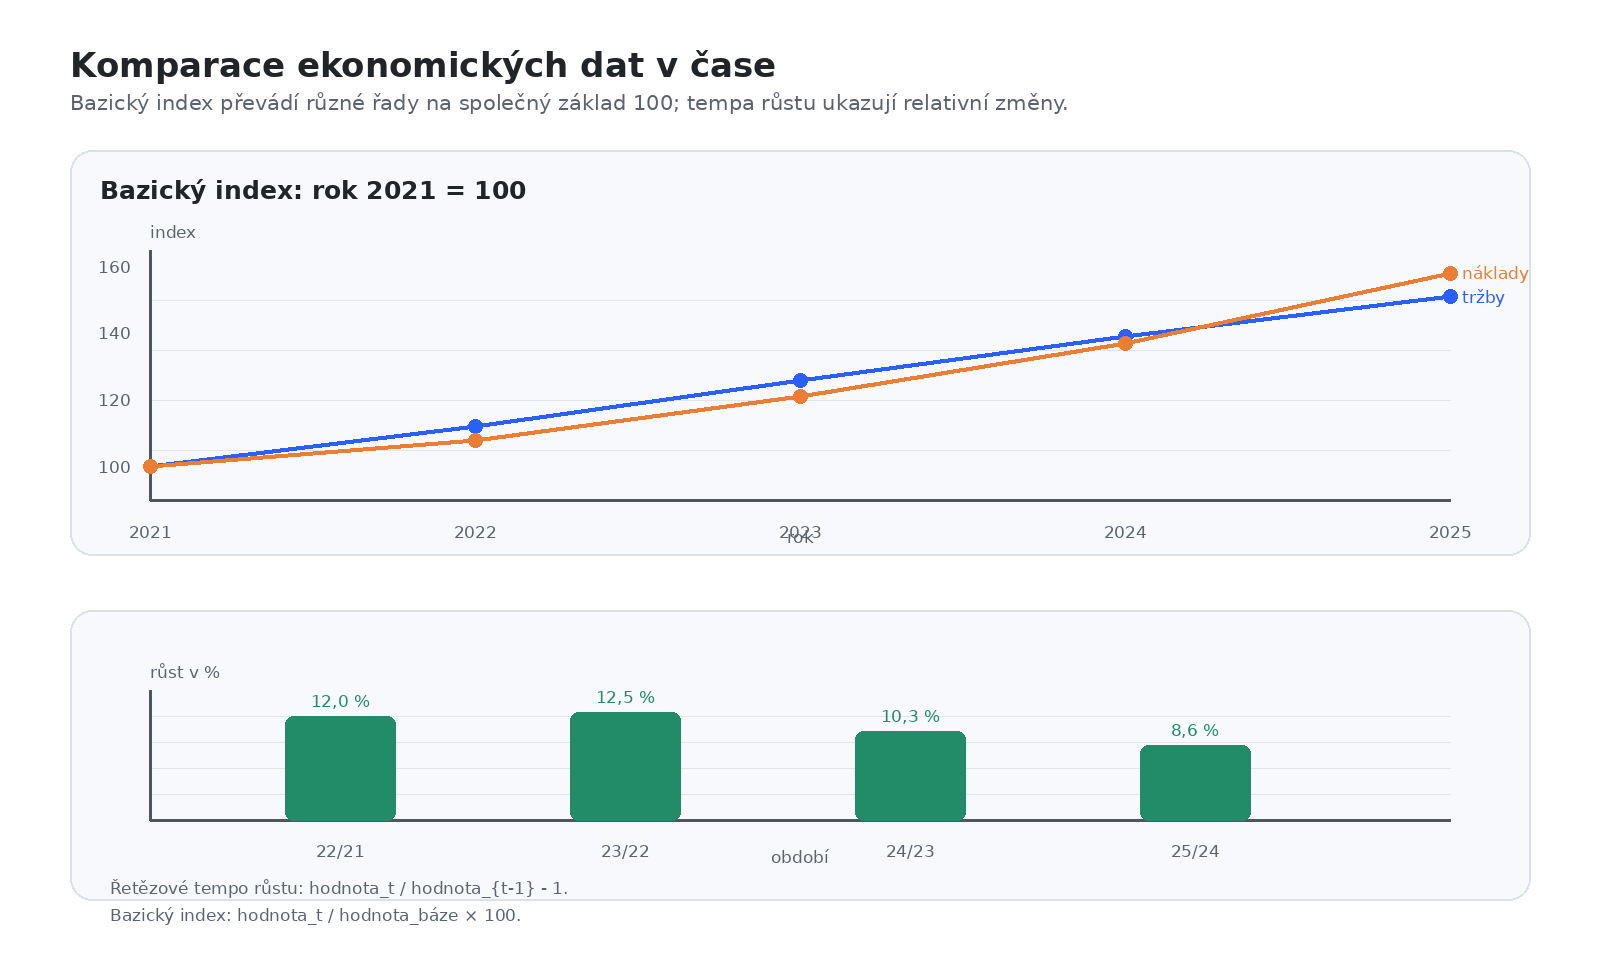
\includegraphics[width=0.95\linewidth]{assets/images/deskriptivni-statistika/economic-comparison-indices.png}
  \caption[Bazický index a tempa růstu]{Komparace ekonomických dat pomocí bazického indexu a řetězových
  temp růstu. Popis obrázku: horní panel převádí tržby a náklady na společný základ 2021 = 100, dolní
  panel ukazuje řetězová tempa růstu mezi sousedními obdobími. Zdroj obrázku: vlastní schéma.}
  \label{fig:economic-comparison-indices}
\end{figure}

U ekonomické komparace je potřeba hlídat:
\begin{itemize}
  \item zda jde o nominální nebo reálné hodnoty očištěné o cenovou změnu;
  \item zda jsou období stejně dlouhá a srovnatelná;
  \item zda sezonnost nezkresluje meziměsíční porovnání;
  \item zda se nezměnila definice ukazatele, datový zdroj nebo metodika;
  \item zda se procentní body nezaměňují s procenty.
\end{itemize}

Příklad rozdílu mezi procenty a procentními body: pokud podíl vzrostl z 10\% na 12\%, zvýšil se o
2 procentní body, ale relativně o 20\%.

U souhrnných cenových a objemových indexů je dobré znát rozdíl mezi \term{Laspeyresovým} indexem
s vahami ze základního období, \term{Paascheho} indexem s vahami běžného období a \term{Fisherovým}
indexem jako jejich geometrickým průměrem. V praxi se tím řeší, zda změnu cen měříme při staré nebo
aktuální struktuře spotřeby či produkce.

V reportingu se často používá i časová komparace typu \term{YTD} -- kumulace od začátku roku do
aktuálního období -- a \term{YoY}, tedy meziroční srovnání stejného období. U sezonných dat je YoY
často smysluplnější než prosté porovnání s bezprostředně předchozím měsícem.

\subsection*{Kontingenční analýza a vztahy mezi proměnnými}
Deskriptivní analýza nemusí popisovat jen jednu proměnnou. Často sleduje vztah dvou proměnných.

\term{Kontingenční tabulka} zobrazuje četnosti kombinací dvou kategoriálních proměnných, například
regionu a typu zákazníka. Z ní lze počítat řádková procenta, sloupcová procenta a celkové podíly.
Řádková procenta odpovídají na otázku \uv{jaká je struktura uvnitř řádku}, sloupcová procenta na
otázku \uv{jak se skládá daný sloupec}.

U dvou kvantitativních proměnných se často používá \term{korelace}. Pearsonův korelační koeficient
popisuje lineární vztah, Spearmanova korelace vztah pořadí. Korelace je deskriptivní míra asociace,
ne důkaz kauzality.

U kombinace kvantitativní a kategoriální proměnné se porovnávají skupinové statistiky: průměr, medián,
IQR, směrodatná odchylka a počet pozorování v každé skupině. Graficky se hodí boxplot nebo sloupcový
graf s intervaly nejistoty, pokud chceme ukázat i spolehlivost odhadu.

\subsection*{Základy statistické inference a testování hypotéz}
Deskriptivní statistika popisuje pozorovaná data. Často ale chceme udělat krok dál: z výběru usuzovat
na širší populaci nebo rozhodnout, zda pozorovaný rozdíl může být jen náhodná výběrová chyba. K tomu
slouží \term{statistická inference}.

Základní rozlišení:
\begin{itemize}
  \item \term{populace} je celek, o kterém chceme něco říct, například všichni zákazníci firmy;
  \item \term{výběr} je pozorovaná část populace, například zákazníci v konkrétním dotazníku;
  \item \term{parametr} je neznámá vlastnost populace, například skutečný průměr \(\mu\);
  \item \term{statistika} je hodnota spočítaná z výběru, například výběrový průměr \(\bar{x}\).
\end{itemize}

Výběrová statistika je zatížená nejistotou. Proto se kromě bodového odhadu často uvádí
\term{standardní chyba}:
\[
  SE(\bar{x})=\frac{s}{\sqrt{n}}.
\]
Čím větší je výběr a čím menší je variabilita dat, tím menší je standardní chyba.

\subsubsection*{Interval spolehlivosti}
Interval spolehlivosti ukazuje rozumný rozsah hodnot populačního parametru. Pro průměr se často zapisuje:
\[
  \bar{x}\pm t_{1-\alpha/2,n-1}\frac{s}{\sqrt{n}}.
\]
U 95\% intervalu volíme \(\alpha=0{,}05\). Širší interval znamená větší nejistotu. Důležité je neříkat,
že \uv{parametr má 95\% pravděpodobnost ležet v tomto konkrétním intervalu}. Ve frekvenční interpretaci
by při opakovaném stejném postupu dlouhodobě přibližně 95\% takto vytvořených intervalů obsahovalo
skutečný parametr.

\subsubsection*{Postup testování hypotéz}
Testování hypotéz převádí věcnou otázku na statistické rozhodnutí.

Typický postup:
\begin{enumerate}
  \item formulovat nulovou hypotézu \(H_0\), obvykle \uv{žádný rozdíl} nebo \uv{žádný efekt};
  \item formulovat alternativu \(H_1\), například oboustrannou \( \mu \neq \mu_0 \) nebo jednostrannou
  \( \mu > \mu_0 \);
  \item zvolit hladinu významnosti \(\alpha\), často 0{,}05;
  \item spočítat testovou statistiku;
  \item určit \(p\)-value nebo porovnat testovou statistiku s kritickou hodnotou;
  \item rozhodnout, zda \(H_0\) zamítáme, a hlavně výsledek věcně interpretovat.
\end{enumerate}

\term{\(p\)-value} je pravděpodobnost, že bychom při platnosti nulové hypotézy pozorovali stejně
extrémní nebo extrémnější testovou statistiku, než jakou jsme dostali v datech. Pokud:
\[
  p\text{-value}<\alpha,
\]
zamítáme \(H_0\) na hladině významnosti \(\alpha\).

Pozor: \(p\)-value není pravděpodobnost, že je nulová hypotéza pravdivá. Také neříká, jak velký nebo
prakticky důležitý je efekt. Malé \(p\)-value může vzniknout u velmi malého, ale přesně odhadnutého
rozdílu ve velkém vzorku.

\subsubsection*{Chyby prvního a druhého druhu}
Při testování můžeme udělat dva základní typy chyb:
\begin{itemize}
  \item \term{chyba I. druhu} - zamítneme pravdivou \(H_0\); její pravděpodobnost kontroluje
  \(\alpha\);
  \item \term{chyba II. druhu} - nezamítneme \(H_0\), i když je ve skutečnosti nepravdivá;
  \item \term{síla testu} je pravděpodobnost správně zamítnout nepravdivou \(H_0\).
\end{itemize}

Snížení \(\alpha\) zmenšuje riziko falešně pozitivního závěru, ale při stejném rozsahu dat obvykle
zvyšuje riziko, že skutečný efekt neodhalíme.

\subsubsection*{t-test}
\term{t-test} se používá hlavně pro testování průměrů, když neznáme populační rozptyl a pracujeme s
výběrovou směrodatnou odchylkou.

Jednovýběrový t-test:
\[
  H_0:\mu=\mu_0,
  \qquad
  t=\frac{\bar{x}-\mu_0}{s/\sqrt{n}}.
\]

Dvouvýběrový t-test porovnává průměry dvou nezávislých skupin:
\[
  H_0:\mu_1-\mu_2=0.
\]
V praxi se často používá Welchův t-test, protože nevyžaduje stejný rozptyl ve skupinách:
\[
  t=
  \frac{\bar{x}_1-\bar{x}_2}
  {\sqrt{s_1^2/n_1+s_2^2/n_2}}.
\]

Párový t-test se používá, když máme dvojice pozorování, například stejný zákazník před a po změně
ceny. Potom testujeme průměr rozdílů:
\[
  d_i=x_{i,\text{po}}-x_{i,\text{před}},
  \qquad
  H_0:\mu_d=0.
\]

Před t-testem je potřeba vědět, co přesně jsou skupiny, zda jsou pozorování nezávislá, zda nejde o
párová data a zda extrémy nebo silná šikmost nedělají průměr zavádějícím.

\subsubsection*{F-test}
\term{F-test} používá testovou statistiku s F-rozdělením. Typicky vzniká jako poměr dvou odhadů
rozptylu nebo jako porovnání vysvětlené a nevysvětlené variability.

Test shody dvou rozptylů:
\[
  H_0:\sigma_1^2=\sigma_2^2,
  \qquad
  F=\frac{s_1^2}{s_2^2}.
\]
Tento test je citlivý na odchylky od normality. Pokud jsou data šikmá nebo mají těžké ocasy, bývá
vhodnější robustnější test rovnosti rozptylů, například Leveneho test.

V analýze rozptylu (ANOVA) se F-test používá k porovnání více skupinových průměrů:
\[
  H_0:\mu_1=\mu_2=\cdots=\mu_g.
\]
Princip je porovnat variabilitu mezi skupinami s variabilitou uvnitř skupin:
\[
  F=\frac{\text{variabilita mezi skupinami}}{\text{variabilita uvnitř skupin}}.
\]
Velké \(F\) znamená, že rozdíly mezi skupinovými průměry jsou velké vzhledem k běžné variabilitě uvnitř
skupin.

V regresi se F-test používá také pro společnou významnost více koeficientů, například zda několik
vysvětlujících proměnných jako celek zlepšuje model. Zkouškově je důležité vědět, že t-test se často
ptá na jeden parametr, zatímco F-test se často ptá na více omezení najednou.

\subsection*{Chybějící hodnoty a kvalita dat}
Deskriptivní analýza má začít kontrolou kvality dat. Bez ní mohou být všechny statistiky formálně
správné, ale věcně zavádějící.

Kontroluje se hlavně:
\begin{itemize}
  \item počet řádků a unikátních identifikátorů;
  \item duplicity;
  \item chybějící hodnoty podle proměnných a skupin;
  \item neplatné kategorie a hodnoty mimo povolený rozsah;
  \item extrémní hodnoty;
  \item jednotky, měny, časová pásma a formáty;
  \item konzistence mezi souvisejícími poli, například datum objednávky před datem doručení.
\end{itemize}

Chybějící hodnoty nelze řešit mechanicky. Je rozdíl mezi \uv{neznámé}, \uv{nevztahuje se},
\uv{odmítnuto odpovědět} a \uv{chyba importu}. Před imputací nebo odstraněním je potřeba zjistit,
zda chybění není systematické, například častější u určitého regionu nebo segmentu.

\subsection*{Praktický postup deskriptivní analýzy}
Typický postup:
\begin{enumerate}
  \item vymezit analytickou otázku, jednotku pozorování a cílové publikum;
  \item zkontrolovat strukturu dat, typy proměnných, jednotky a chybějící hodnoty;
  \item spočítat základní četnosti a souhrnné statistiky;
  \item zobrazit rozdělení klíčových proměnných histogramem, boxplotem nebo hustotou;
  \item porovnat hodnoty podle hlavních dimenzí;
  \item ověřit agregace, váhy a definice odvozených metrik;
  \item interpretovat výsledky věcně, ne jen mechanicky podle čísel;
  \item zdokumentovat zdroj, období, filtry, definice a omezení.
\end{enumerate}

\subsection*{Nástroje}
Deskriptivní statistiku lze dělat v tabulkových procesorech, databázích, programovacích jazycích
i BI nástrojích.

\begin{center}
\small
\begin{tabular}{@{}>{\raggedright\arraybackslash}p{0.24\textwidth}
                >{\raggedright\arraybackslash}p{0.30\textwidth}
                >{\raggedright\arraybackslash}p{0.35\textwidth}@{}}
\hline
\term{Nástroj} & \term{Příklady funkcí} & \term{Typické použití} \\
\hline
Excel / Google Sheets & kontingenční tabulky, \texttt{AVERAGE}, \texttt{MEDIAN}, grafy & rychlé
ad hoc přehledy a menší datové sady \\
SQL & \texttt{GROUP BY}, \texttt{COUNT}, \texttt{SUM}, \texttt{AVG}, \texttt{MIN}, \texttt{MAX} &
agregace přímo v databázi \\
Python & pandas \texttt{describe}, \texttt{groupby}, \texttt{pivot\_table}; seaborn, matplotlib &
opakovatelná analýza, větší datové sady, notebooky \\
R & \texttt{summary}, \texttt{aggregate}, \texttt{dplyr}, \texttt{ggplot2} & statistická analýza
a publikovatelné grafy \\
BI nástroje & Power BI, Tableau, Qlik & dashboardy, KPI, drill-down, sdílené reporty \\
\hline
\end{tabular}
\end{center}

\pozor
Nejčastější chyba u zkoušky je vyjmenovat průměr, medián a směrodatnou odchylku bez kontextu. Správná
odpověď musí říct, kdy která statistika dává smysl, jak ji ovlivňují extrémy, jak se agregují metriky
a jak se porovnávají ekonomická data. Druhá častá chyba je průměrovat poměry bez vah nebo zaměnit
procenta a procentní body.

U testování hypotéz je nejčastější chyba říct, že \(p\)-value je pravděpodobnost platnosti nulové
hypotézy. Není. Je to pravděpodobnost tak extrémní testové statistiky za předpokladu, že \(H_0\) platí.
Statistická významnost také není totéž co věcná významnost. U velkých dat může být i malý a prakticky
nevýznamný rozdíl statisticky významný.

\subsection*{Shrnutí ke zkoušce}
\begin{itemize}
  \item Deskriptivní analýza popisuje již pozorovaná data; neprokazuje kauzalitu a sama o sobě
  nepredikuje budoucnost.
  \item Volba statistiky závisí na typu proměnné: nominální, ordinální, intervalové nebo poměrové.
  \item Četnostní analýza pracuje s absolutními, relativními a kumulativními četnostmi.
  \item Míry polohy zahrnují průměr, vážený průměr, medián, modus a kvantily.
  \item Míry variability zahrnují rozpětí, rozptyl, směrodatnou odchylku, IQR a variační koeficient.
  \item Medián, IQR a MAD jsou robustnější vůči extrémům než průměr a směrodatná odchylka.
  \item Histogram a boxplot pomáhají odhalit šikmost, těžké ocasy, vícemodalitu a odlehlé hodnoty.
  \item Agregace vyžaduje správnou granularitu, dimenze, metriky a agregační funkce.
  \item Poměrové ukazatele je často nutné počítat z agregovaných čitatelů a jmenovatelů, ne jako
  prostý průměr procent.
  \item Ekonomická data se porovnávají absolutní změnou, relativní změnou, bazickými a řetězovými
  indexy, tempy růstu a benchmarky.
  \item U interpretace je nutné hlídat kvalitu dat, chybějící hodnoty, změny metodiky, sezonnost,
  inflaci a srovnatelnost období.
  \item Základní inferenční postup rozlišuje populaci, výběr, parametr, statistiku, standardní chybu,
  interval spolehlivosti a test hypotézy.
  \item \(p\)-value porovnává pozorovaný výsledek s tím, co by bylo očekávatelné při platnosti nulové
  hypotézy; malé \(p\)-value samo o sobě neříká, že efekt je velký nebo kauzální.
  \item t-test se používá hlavně pro testování průměrů; F-test pro poměry rozptylů, ANOVA a společné
  testování více omezení.
\end{itemize}

\subsection*{Zdroje}
\begin{itemize}
  \item NIST/SEMATECH e-Handbook of Statistical Methods: \href{https://itl.nist.gov/div898/handbook/eda/eda.htm}{Exploratory Data Analysis}.
  \item NIST/SEMATECH e-Handbook of Statistical Methods: \href{https://www.itl.nist.gov/div898/handbook/eda/section3/eda351.htm}{Measures of Location}.
  \item NIST/SEMATECH e-Handbook of Statistical Methods: \href{https://www.itl.nist.gov/div898/handbook/eda/section3/eda356.htm}{Measures of Scale}.
  \item NIST/SEMATECH e-Handbook of Statistical Methods: \href{https://www.itl.nist.gov/div898/handbook/eda/section3/histogra.htm}{Histogram}.
  \item NIST/SEMATECH e-Handbook of Statistical Methods: \href{https://www.itl.nist.gov/div898/handbook/eda/section3/boxplot.htm}{Box Plot}.
  \item NIST/SEMATECH e-Handbook of Statistical Methods: \href{https://www.itl.nist.gov/div898/handbook/eda/section3/eda35b.htm}{Measures of Skewness and Kurtosis}.
  \item NIST/SEMATECH e-Handbook of Statistical Methods: \href{https://www.itl.nist.gov/div898/handbook/prc/section1/prc131.htm}{Critical values and p values}.
  \item NIST/SEMATECH e-Handbook of Statistical Methods: \href{https://itl.nist.gov/div898/handbook/eda/section3/eda359.htm}{F-Test for Equality of Two Variances}.
  \item NIST Dataplot Reference Manual: \href{https://www.itl.nist.gov/div898/software/dataplot/refman1/auxillar/t\_test.htm}{T TEST}.
  \item PennState STAT 500: \href{https://online.stat.psu.edu/stat500/Lesson06.html}{Hypothesis Testing}.
  \item R Documentation: \href{https://stat.ethz.ch/R-manual/R-devel/library/stats/html/IQR.html}{The Interquartile Range}.
  \item OECD: \href{https://www.oecd.org/en/publications/oecd-glossary-of-statistical-terms_9789264055087-en.html}{OECD Glossary of Statistical Terms}.
\end{itemize}

\newpage
